\section{Results}

\subsection{Quantitative results}
The main quantitative results are presented in \mbox{Table \ref{tab:main_exp}}. PRIDE outperforms all baselines by a large margin, including other BERT-based models.
Unlike BERT$_{ddrel}$, which aggregates predictions on conversation snippets outside of the model, PRIDE internally learns the conversation representation.
Furthermore, unlike BERT$_{conv}$, we do not crop the input sequence to 512 token limit and make use of the hierarchical structure of the conversations.

\begin{table}[]
\centering
\begin{adjustbox}{width=0.7\textwidth}
\begin{tabular}{@{}llllllll@{}}
 & \multicolumn{3}{c}{cross-val on FiRe} & \multicolumn{4}{c}{train:FiRe, test:Series} \\
 \cmidrule(lr){2-4} \cmidrule(lr){5-8}
\textbf{model}           & \textbf{F1}   & \textbf{precision} & \textbf{recall} & &  \textbf{F1}   & \textbf{precision} & \textbf{recall} \\ \toprule
RNN             & 0.11 & 0.11      & 0.15  & & 0.10 & 0.17 & 0.14 \\
BERT$_{ddrel}$ & 0.20 & 0.20      & 0.25   & & 0.14 & 0.22 & 0.15 \\
HAM             & 0.23 & 0.25      & 0.22  & & 0.16 & 0.21 & 0.16 \\
BERT$_{conv}$  & 0.27 & 0.25      & 0.33   & & 0.25 & 0.35 & 0.21 \\ \midrule
PRIDE           & \textbf{0.38} & \textbf{0.42}      & \textbf{0.37} & & \textbf{0.30} & \textbf{0.43}      & \textbf{0.29}\\
\end{tabular}
\end{adjustbox}
\caption{Results on FiRe and Series datasets. The best scores (bold) significantly differ from the remaining ones measured by a McNemar’s test (p $<$ 0.05).}
\label{tab:main_exp}
\end{table}

We also analyze PRIDE's transfer learning performance on the Series dataset as our test data. 
From the results shown in Table \ref{tab:main_exp}, we observe the same behaviour of the models, with PRIDE outperforming the baselines. 
F1 scores are generally lower than the evaluation on the FiRe dataset, 
due to the different nature of data (longer input sequences). 
PRIDE's precision is similar on both datasets, but the larger amount of input utterances with Series seems to reduce recall.

\subsection{Comparison with human performance}

%Even humans often struggle to correctly identify the relationship between the speakers of a given conversation.
It is often complicated even for humans to recognize the relationship between the speakers in a given conversation. 
Thus, human performance can be regarded as an upper bound on the model's performance. 
To obtain this upper bound estimation, we asked three human annotators to read the complete conversation history of two movie characters (the same as the input given to the model) and identify the applicable relationships.
%(This differs from our main dataset because annotations are based on conversations rather than on character descriptions.)
We sampled 5 pairs for each relationship label, resulting in 60 pairs. As human-predicted labels we assigned the relationships selected by at least 2 out of 3 annotators.
The results on this dataset are shown in Table \ref{tab:human_exp}.
While PRIDE substantially outperforms the baselines, it achieves about half of human precision, illustrating the difficulty of the given task.


\begin{table}[]
\centering
\begin{adjustbox}{width=0.43\textwidth}
\begin{tabular}{@{}llll@{}}
\textbf{model}           & \textbf{F1}   & \textbf{precision} & \textbf{recall} \\ \toprule
RNN        & 0.04     & 0.02            & 0.10          \\
BERT$_{ddrel}$ & 0.15     & 0.15            & 0.20          \\
HAM        & 0.24     & 0.30             & 0.23         \\
BERT$_{conv}$  & 0.23     & 0.32            & 0.23         \\
PRIDE      & \textbf{0.33}     & \textbf{0.41}            & \textbf{0.35}         \\ \midrule
human      & 0.84     & 0.89            & 0.79        
\end{tabular}
\end{adjustbox}
\caption{Results on a human-annotated FiRe subset.}
\label{tab:human_exp}
\end{table}

\subsection{Ablation study}

To investigate the impact of different components of PRIDE on its performance,
we run an ablation study, removing one PRIDE component at a time: we experimented on excluding additional age and interpersonal dimensions' representations as well as removing speaker and positional embeddings from Transformer's input.
The ablation on Transformer is done by substituting it with aggregation operations on word and utterance levels consecutively. 
Results are shown in Table \ref{tab:ablation}. 
It can be observed that removing positional encoding gives the least impact. On the other hand, the quality considerably drops by removing Transformer, which is caused by a very low recall. Removing other elements cause a drop in precision, suggesting that incorporating age differences and interpersonal dimensions improves performance.

\begin{table}[t!]
\centering
\begin{adjustbox}{width=0.53\textwidth}
\begin{tabular}{@{}llll@{}}
\textbf{model}           & \textbf{F1}   & \textbf{precision} & \textbf{recall} \\ \toprule
PRIDE               & \textbf{0.38}     & 0.42            & 0.37         \\ \midrule
PRIDE $-$ dimensions  & 0.36     & 0.36            & 0.40          \\
PRIDE $-$ age         & 0.37     & 0.38            & 0.37         \\
PRIDE $-$ speaker     & 0.35     & 0.37            & 0.36         \\
PRIDE $-$ positional  & 0.37     & 0.36            & \textbf{0.41}         \\
PRIDE $-$ Transformer* & 0.35     & \textbf{0.46}            & 0.33        
\end{tabular}
\end{adjustbox}
\caption{Ablating elements of PRIDE. The models marked with * significantly differ with full PRIDE, measured by a McNemar’s test (p $<$ 0.05). 
}
\label{tab:ablation}
\end{table}

\subsection{Varying input length}

\begin{figure}[t!]
\centering
\begin{adjustbox}{width=0.65\textwidth}
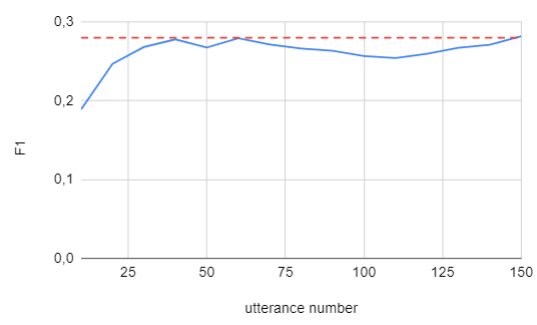
\includegraphics[0.5\textwidth]{imgs/increasing.PNG}
\vspace*{-0.3cm}
\end{adjustbox}
\caption{F1 when varying input length. The dotted red line shows the performance on the full input.}
\label{increasing}
\end{figure}

To investigate how many utterances are needed to make accurate predictions, we ran the trained PRIDE model on a subset of data with inputs of varying lengths.
To do so, we selected a subset of user pairs with at least 150 utterances, and perform inference while increasing the length of the slice of input utterances from 10 to 150.
This was repeated over 100 runs, with the randomized starting position of the slice.
The results averaged over all runs are shown in Figure \ref{increasing}.
We observe that approximately 40 utterances are enough to maximize performance in terms of F1 score.

\subsection{Per class analysis}

\begin{table}[]
\centering
\begin{adjustbox}{width=0.63\textwidth}
\begin{tabular}{@{}l|c|ccc@{}}
\textbf{class}      & \textbf{count} & \textbf{PRIDE} & \textbf{($-$ speaker)} & \textbf{($-$ dimensions)} \\ \toprule
friend                          & 208                             & 0.50                            & 0.50                                      & 0.50                 \\
lover                           & 187                             & 0.60                            & 0.58                                      & 0.60                 \\
spouse                          & 69                              & 0.40                            & 0.40                                      & 0.35                 \\
colleague                       & 67                              & 0.25                            & 0.25                                      & 0.25                 \\
child                           & 48                              & 0.60                            & 0.51                                      & 0.56                 \\
parent                          & 41                              & 0.62                            & 0.55                                      & 0.60                 \\
sibling                         & 37                              & 0.42                            & 0.33                                      & 0.40                  \\
employee                        & 34                              & 0.29                            & 0.23                                      & 0.26                 \\
boss                            & 29                              & 0.04                            & 0.08                                      & 0.04                 \\
enemy                           & 27                              & 0.14                            & 0.13                                      & 0.14                 \\
medical                         & 19                              & 0.46                            & 0.47                                      & 0.44                 \\
commercial                      & 19                              & 0.12                            & 0.12                                      & 0.06            
\end{tabular}
\end{adjustbox}
\caption{Class F1 scores of PRIDE and PRIDE without speaker embeddings and interpersonal dimensions.}
\label{perclass}
\end{table}

In Table \ref{perclass} we show the label distribution and per class F1 scores for PRIDE and two ablated versions.
We observe that using speaker embeddings benefit predictions on asymmetric classes, such as \emph{child} and \emph{parent}, as their F1 scores drop significantly when speaker embeddings are not used. Removing interpersonal dimensions damages performance on \textit{spouse} and \textit{child} in particular, illustrating  how this signal can help differentiate relationships that use similar vocabulary.


\subsection{Misclassification analysis}

\begin{figure}[t!]
\centering
\begin{adjustbox}{width=0.6\textwidth}
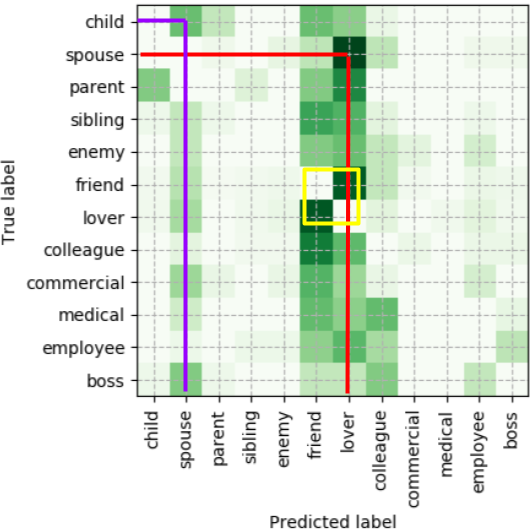
\includegraphics[0.3\textwidth]{imgs/confusion_marked.png}
\vspace*{-0.3cm}
\end{adjustbox}
\caption{Confusion matrix}
\label{confusion}
\end{figure}

The confusion matrix for PRIDE's predictions is shown in Figure \ref{confusion}. To create the confusion matrix for the multi-label case, we consider only incorrect predictions (either the labels which the model omitted or which it falsely predicted). For a single test instance we remove true positives from its sets of correct and predicted labels and use the Cartesian product of these sets to build the matrix.

We observe that there are many misclassifications into the \emph{friend} and \emph{lover} labels, which are the most common (see columns).
This can be attributed to the model's tendency to predict majority classes because of a considerable class imbalance. 

Considering specific pairs, we see that the model often confuses \emph{spouse} for \emph{lover} (red line). They may talk to each other in a similar tone and use the same address terms. Conceptually, however, these classes are different, with spouses having tighter family bonds, discussing children and household issues, and lovers talking more casually.
Similarly, \emph{child} and \emph{spouse} are often confused as well (purple line). Both may use terms related to family and discuss similar topics. The differences between \emph{lover} and \emph{friend} are indeed subtle (yellow square), and these pairs were also sometimes confused by human annotators.

Finally, we investigated the impact of confusion within asymmetric classes (for example, confusing \emph{parent} to \emph{child}). We found that if we accept the model's predictions of either label as correct, the average number of false positives for such classes drops by 34\%, resulting in an increase in average F1 score from 0.38 to 0.43.
This illustrates the challenge posed by considering relationship directions and the importance of including asymmetric labels.

